			
\section{Adversarial Search and Games}
	\subsection{Game}
		Un environnement multiagent peut etre vu comme un jeu et donc un problème résolut par recherche.
		
		On va parler de \textbf{Zero-sum} qui veut dire que si un mouvement avantage un joueur alors il n'avantages pas l'autre joueur. le jeux possède un seul gaganant et un seul perdant, pas de neutre ou 2 gagnants ou 2 perdants.
		
		
		Un jeux est défini par :
		\begin{itemize}
			\item \textbf{Initial state} : $S_0$ positions de début du jeu
			\item \textbf{To-Moce(s)} : Le joueur qui doit jouer au state $s$
			\item \textbf{Actions(s)} : ensemble des mouvement légaux qu'il a fait en state $s$
			\item \textbf{Result(s,a)} : modèle de transition, state final après actions $a$ sur le state $s$
			\item \textbf{Is-Terminal(s)} : test terminal du state $s$, si la partie est finie
			\item \textbf{Utility(s,p)} :  valeur numérique du résultat du jeux  en au state $s$ pour le player $p$
		\end{itemize}	
		
		
		\textit{Initial states}, \textit{Actions(s)} et \textit{Results(s,a)} definisse le \textit{State space search} et le tree du jeux.
	\subsection{MinMax Algo}
	
		\begin{figure}[htp]
			\centering
			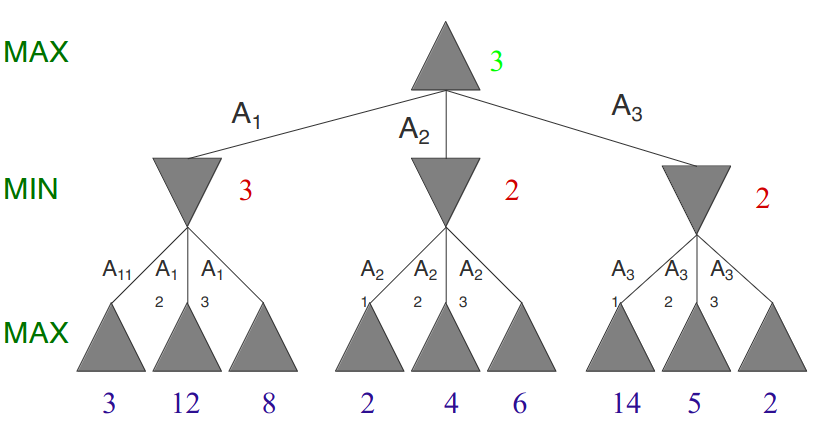
\includegraphics[width=0.7\textwidth]{img/minmax.png}
		\end{figure}
		
		Optimal pour les jeux déterministe et a 2 joueurs. 
		
		Chaque niveau représente à un joueur de jouer en fonction du state, un joueur (MAX) veut maximiser la valeur le deuxième joueur (MIN) lui veut minimiser. Si un des joueurs ne joue pas de maniéré optimale alors l'autre joueur va encore mieux en profiter et en ressortir un meilleur score.
		
		MinMax génère le tree entièrement et applique une fonction d'utilité sur les derniers state (les leafs de l'arbre). Ensuite on remontre l'arbre en choisissant le MIN ou le MAX value en fonction du niveau de l'arbre (tours du joueurs). Le node final au dessus représente le meilleur mouvement possible

		\begin{figure}[htp]
			\centering
			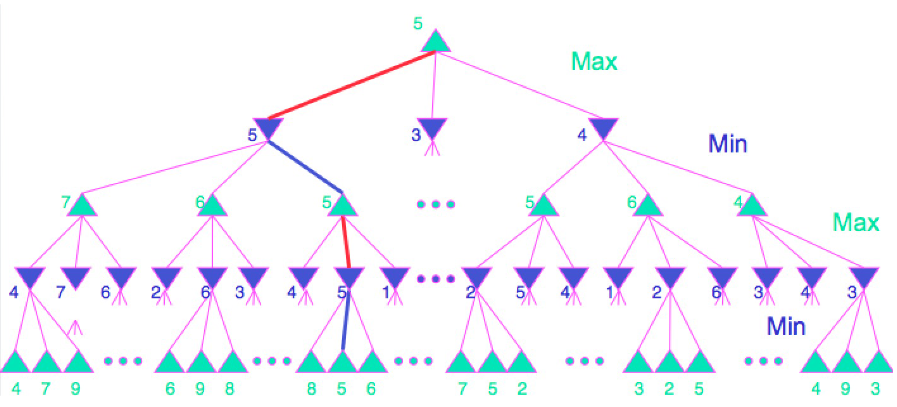
\includegraphics[width=0.7\textwidth]{img/exMinMax.png}
			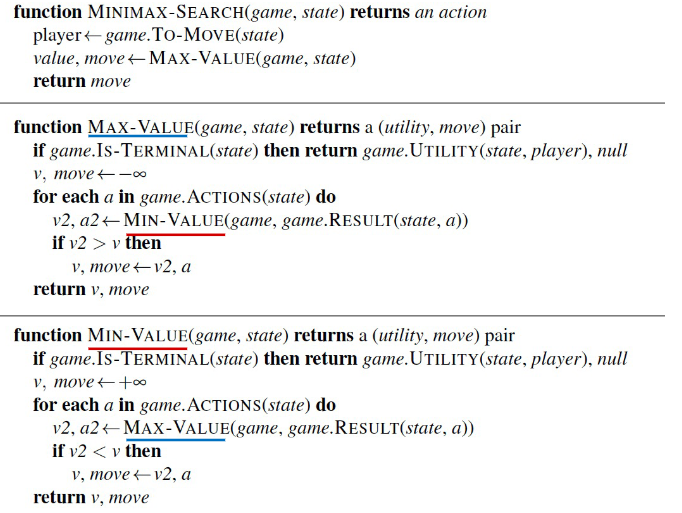
\includegraphics[width=0.7\textwidth]{img/algoMinMax.png}
		\end{figure}

		
		Il est possible de modifer l'algo pour avoir plus de 2 joueurs, il suffit de garder un vecteur a chaque node ou les élements du vecteur sont les utilité de chaque joueurs. Chaque joueur va choisir le mouvement qui maximise l'utilité
		
		Propriétés :
		\begin{itemize}
			\item Basé sur DFS (recursif)
			\item \textbf{Complete} si l'arbre est fini
			\item \textbf{Time complexity} : $\mathcal{O}(b^m)$
			\item \textbf{Space complexity} : $\mathcal{O}(bm)$
		\end{itemize}
		
	\subsection{Alpha-Beta pruning}
		On cherche a "élagué" l'arbre afin de retirer les branche au quelle nous somme sur que il n'y a pas de meilleurs valeurs et donc inutile.Il n'affecte pas le resultat final
		\begin{figure}[H]
			\centering
			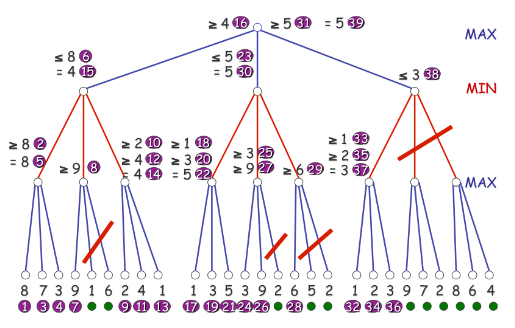
\includegraphics[width=0.7\textwidth]{img/alphabeta.png}
		\end{figure}
		
		\begin{figure}[H]
			\centering
			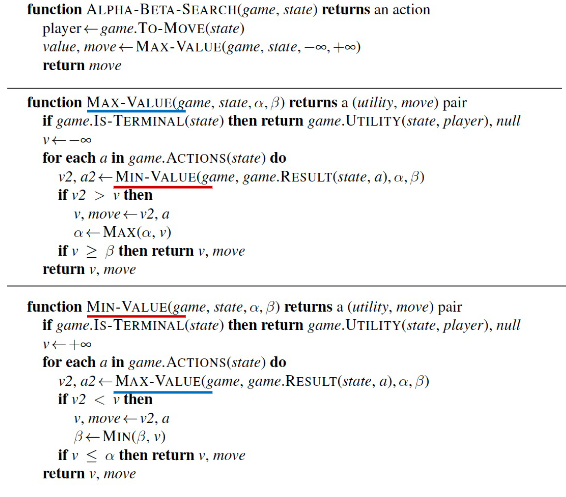
\includegraphics[width=0.7\textwidth]{img/alphabetaalgo.png}
		\end{figure}
		
		$\alpha$ : Valeur du meilleur (plus grande) choix trouvé d'ici la depuis les path visité pour MAX
		
		$\beta$ : Valeur du meilleur (plus petit) choix trouvé d'ici la depuis les path visité pour MIN
		
		Si les sucesseur de l'arbre sont idéalement visité, la complexité temporelle est alors de $\mathcal{O}(b^{d/2})$ et si visité random $\mathcal{O}(b^{3d/4})$
		
		Voila un autre exemple de prunning car un peu dure a comprendre parfois :
		
		\begin{figure}[H]
			\centering
			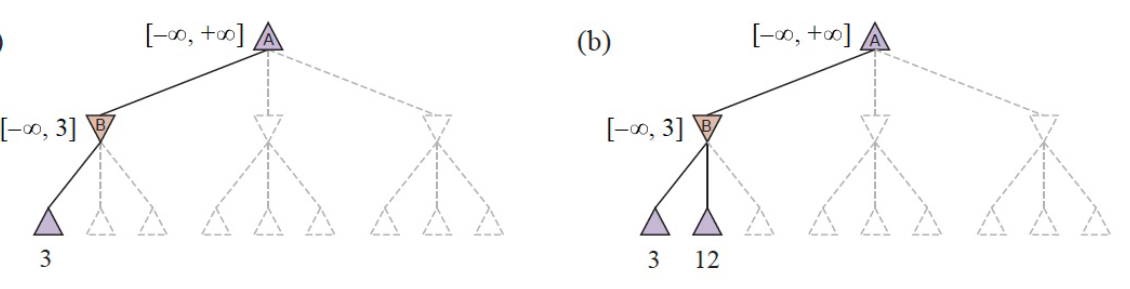
\includegraphics[width=\textwidth]{img/AB.png}
		\end{figure}
		
		\begin{figure}[H]
			\centering
			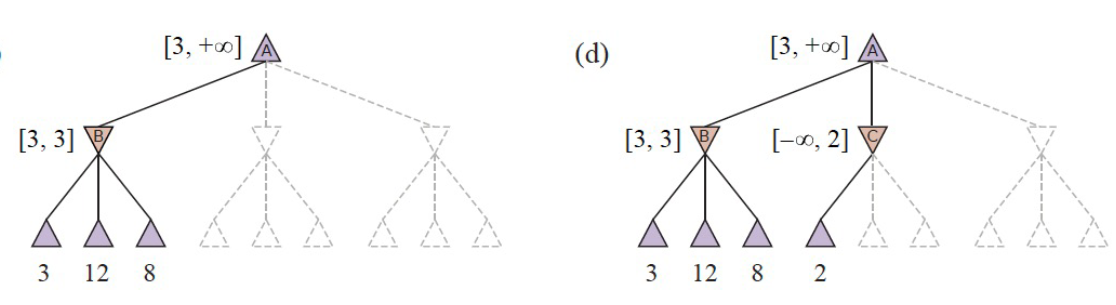
\includegraphics[width=\textwidth]{img/AB1.png}
		\end{figure}
		
		\begin{figure}[H]
			\centering
			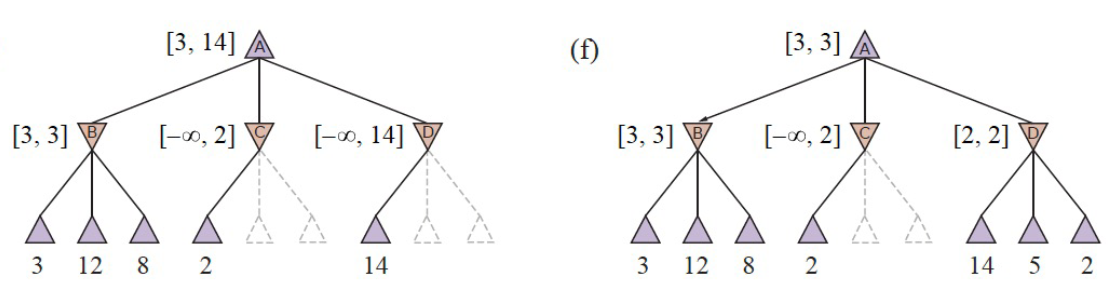
\includegraphics[width=\textwidth]{img/AB2.png}
		\end{figure}
		
		
		\subsubsection{Move ordering}
	
			La disposition des nodes est idéal si le meilleur node est le plus a gauche.
			On peut tenter de réaranger les nodes afin d'avoir les meilleur le plus a gauche, et trouver le \textbf{Killer move}
	\subsection{Imperfect Decisions}
		
		En pratique il est souvent impossible de faire une research complete car trop grand. Ce que on fait, on fait une search dans seulement un partie du graph. Cela requière une fonction  cutoff-test qui indique quand stopper la génération du graph. Mais donc on ne peut pas savoir la valeur de l'utilité des derniers node juste avant le cutoff, on va donc devoir l'estimer avec une fonction heuristique.
		
		\subsubsection{Evaluation Function}
		
			\begin{figure}[H]
				\centering
				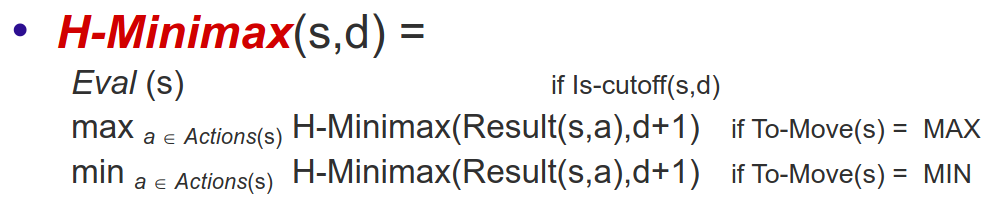
\includegraphics[width=\textwidth]{img/evalF.png}
			\end{figure}

			La fonction doit etre :
			\begin{itemize}
				\item Consistent avec la fonction d'utilité
				\item équilibré entre présicions et temps de calcul
				\item Dois reflétér la réal chance de gagné
				\item Fonction linéaire avec du poid sont souvent 
			\end{itemize}
			
		\subsubsection{Cutting off the search}
		
		On doit un peux changer le code de alpha-Beta-Search qui doit appeler Eval quand il y a un cutoff

		if game.Is-Cutoff(state, depth) then return EVAL(state, player), null
		
			
		La fonction d'évaluation doit être appliquée uniquement à la position quiescentes, c'est-à-dire stables. (qui ne risquent pas de connaître de fortes variations de valeur dans un avenir proche).			
			
			Il y a \textbf{l'effet d'horizon} : Nous pouvons retarder les catastrophes, mais nous ne pouvons pas les prévenir. Cela peut arriver à cause d'une coupure car l'horizon n'est pas assez profond. Si un agent est confronté à un mouvement qui cause de graves dommages et qui est inévitable à la fin, il essaiera de l'éviter le plus longtemps possible. l'éviter le plus longtemps possible. Au bout du compte, il perdra autant, voire plus.
			
		\subsubsection{Forward pruning}
			Quelques moves a certains nodes sont "élagué" direct sans considérations directe, il coupe les moves "mauvais" mais il possible que plus tard se soit le move qui nous fait gagner.
			Avec le \textbf{Beam search}, on considère un ensemble de $n$ mouvement plutôt que le tous les mouvements possibles, on réduit de beaucoup  de temps de calcule "inutile"
			
		\subsubsection{Search VS. Lookup}
			Beaucoup utilise des table lookup (table avec les actions a faire en fonction de la situation) pour le début de la partie. Ca sert a rien de faire un arbre de millions de nodes pour une personne qui a 2/3 de chance de faire E4 au debut. 
		
		Les lookup tables sont donc utilisé en début et fin de game car souvent la meme choses avec des pattern et des solutions déja connue.
			
	\subsection{Monte Carlo Tree Search}
			
		Fonction d'utilité estimée comme l'utilité moyenne (par exemple, pourcentage de victoire) sur des simulations (appelées playout) de jeux complets. On a déja tester avant et on sait le pourcentage de victoire avec ces moves.
		
		Jouer avec des coups légaux aléatoires de la part des deux joueurs
		
		On a un search tree qui augmente a chaque itérations
		\begin{itemize}
			\item \textbf{Selection} : Commence du root et va a une leaf en utilisant une selection de stratégies
			\item \textbf{Expansion} : Ajoute un nouvel enfant au node
			\item \textbf{Simulations} : jouer (sans enregistrer les moves)
			\item \textbf{Back-propagation} : update les parents dans le tree
		\end{itemize}
		
		\begin{figure}[H]
			\centering
			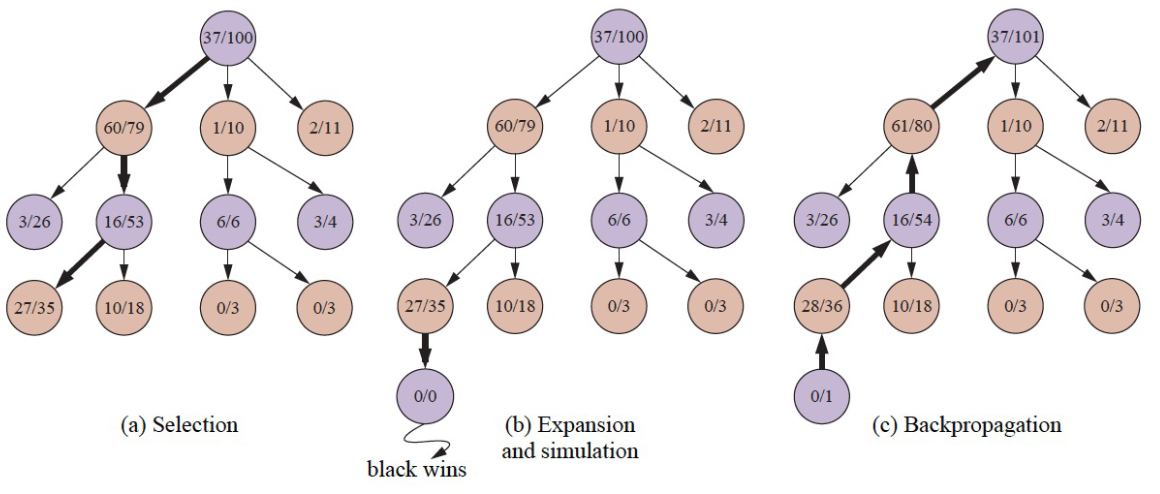
\includegraphics[width=\textwidth]{img/MCTS.png}
		\end{figure}
		
		\begin{figure}[H]
			\centering
			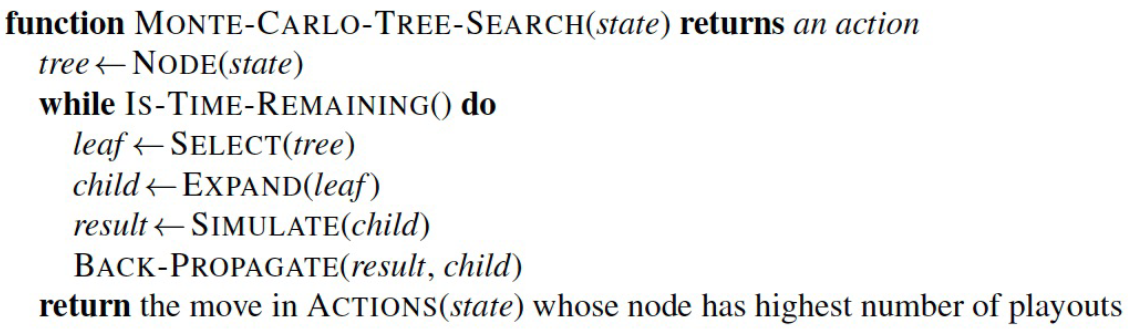
\includegraphics[width=\textwidth]{img/MCTS1.png}
		\end{figure}
	
	\subsection{Stochastic Games}
		Ce sont des jeux avec un degré d'improbabilité parmis les elements randoms. Cela requierd une chance pour chaque nodes en plus des Min Max
		
		
		\subsubsection{Expectminimax}
			Cet algo ajoute de la chance aux nodes en plus de MAX MIN. Complexité de $\mathcal{O}(b^{m}n^{m})$ ou $n$ est le nombre de chance d'event distincte
			
		\begin{figure}[H]
			\centering
			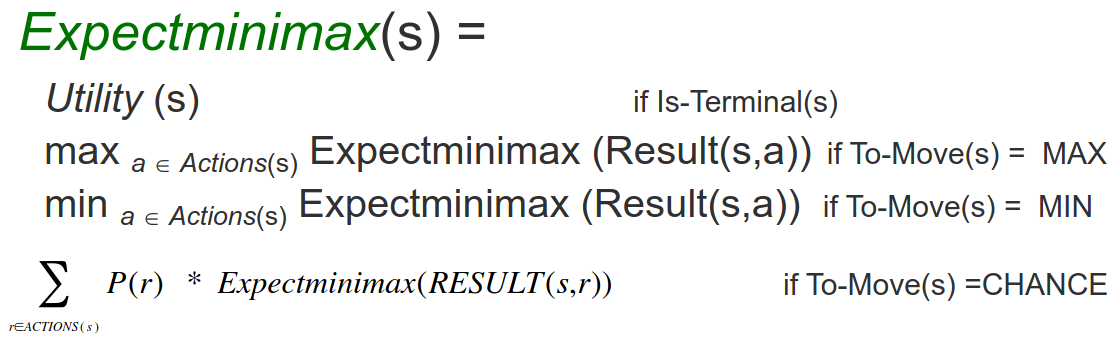
\includegraphics[width=\textwidth]{img/EM.png}
		\end{figure}
		
		On peut pruner dans le meme genre que alpha beta